\chapter{Introduction}
\label{chap:intro}

An online version of this text and repository may be found
\href{https://github.com/chgorman/Notes-Math-Crypto}{here}.



\section{Primary Goal}

These notes introduce cryptography and the necessary mathematics;
the primary focus is \gls{publiccrypto}
with particular emphasis on \gls{ecc} and \glspl{signature}.
The required mathematical maturity is not too great
provided the end goal is to gain a deeper understanding of cryptography.
Ideally, after working through this material, the reader
will understand the pseudocode of cryptographic algorithms
and the ideas behind them.
We note, however, that the discussion here is \emph{woefully insufficient}
to \emph{implement} cryptographic algorithms;
even so, we make an effort to point out
problems that arise in practice.
References are provided throughout for the inquisitive reader.

We note that intra-document links are \textcolor{blue}{blue}
while external links are \textcolor{magenta}{magenta}.
For instance, see Figure~\ref{fig:xkcd_security} for an
\texttt{xkcd} webcomic discussing security
that may be found online at \url{https://xkcd.com/538/}.

\begin{figure}[t]
\centering
    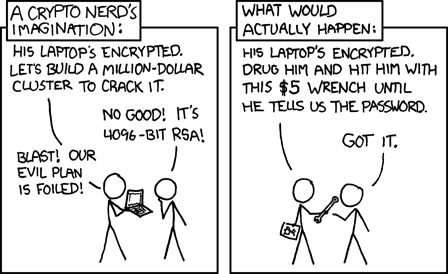
\includegraphics[width=0.75\textwidth]{figures/xkcd/xkcd_538_security.png}
    \caption[\texttt{xkcd} Security]{Here we have an example of cryptography
        in the wild.
        To defend against rubber-hose cryptanalysis,
        see~\cite{bojinov2012neuroscience}.
        Created by Randall Munroe on \texttt{xkcd};
        posted online at \url{https://xkcd.com/538/}.
        }
    \label{fig:xkcd_security}
\end{figure}


These notes may also be helpful to understand the cryptography in the
\href{https://github.com/alicenet/whitepaper}{AliceNet
Whitepaper}~\cite{AliceNetWhitepaper}.
\emph{Full disclosure:} the author of the present work
helped write~\cite{AliceNetWhitepaper}.



\section{Intended Audience}

This document is written for individuals without a significant
background in mathematics.
The necessary mathematics for \gls{publiccrypto} involves
\gls{number theory} and algebra (\gls{group} theory, \gls{field} theory, and
\glspl{elliptic curve}).
The main requirement for learning this material is dedication.

Although this is primarily aimed at software engineers
interested in cryptography,
other technically-inclined individuals may find these notes helpful;
that is, the material presented here is meant to be accessible
to those who studied mathematics,
science, or engineering at the collegiate level.
Individuals who do not meet this criterion are still encouraged
to continue reading if the material is deemed sufficiently interesting.



\section{Examples}

Concrete examples will be used throughout to assist comprehension.
\texttt{Python} scripts are included that may easily be modified;
see \texttt{examples/} and its subdirectories.

We note that \texttt{code/} stores code for printed examples
throughout the text and is not meant to be modified;
this is separate from \texttt{examples/}, which is designed to be modified.


\section{Overview}

In Chapter~\ref{chap:do_not}, we focus on ``what not to do''.
This includes many bad ideas.
The main takeaway is this:
\textbf{do not write your own cryptographic algorithms or protocols}.

We start by introducing the mathematics used
throughout these notes in Chapters~\ref{chap:math_1},
\ref{chap:math_2}, and \ref{chap:math_3};
the material becomes progressively more abstract.
In Chapter~\ref{chap:math_3}, we discuss \glspl{elliptic curve},
\glspl{bilinear}, and \gls{lagrange interpolation};
this may be a bit advanced,
so on the initial reading this chapter may be skipped
and read at a future point in time.

After the mathematical review, we spend some time discussing
\gls{symmetriccrypto} in Chapter~\ref{chap:symmetric}.
This material is probably more familiar:
Alice and Bob share a secret key and want to communicate.
We spend significant time talking about \glspl{hash function};
\glspl{hash function} are first discussed in
Chapter~\ref{chap:hash} while their applications are discussed in
Chapter~\ref{chap:hash_applications}.

At this point, we focus on \gls{publiccrypto}
in Chapter~\ref{chap:public}.
In this case, Alice and Bob use 2 keys to communicate:
one public key and one private key.
We spend Chapter~\ref{chap:signatures} discussing an important
aspect of \gls{publiccrypto}: \glspl{signature}.
After this, we look at \gls{ecc} in Chapter~\ref{chap:elliptic};
this involves reworking material from Chapters~\ref{chap:public}
and \ref{chap:signatures} in terms of \glspl{elliptic curve}.

Starting with Chapter~\ref{chap:pairing} on \gls{pairingcrypto},
the material becomes more advanced.
After this, we discuss \glspl{zkproof} in Chapter~\ref{chap:zkproofs}.
To wrap up, we end with a discussion of secret sharing protocols
and \gls{distributed key generation} in Chapter~\ref{chap:secret_sharing};
the discussion here draws on material from essentially \emph{all}
of the previous chapters.

In Chapter~\ref{chap:hardness}, we discuss some of the hardness assumptions
in \gls{publiccrypto}.
If certain mathematical problems are hard to solve,
then the cryptographic protocols discussed here are secure.



\section{Cryptographic Participants}

We will frequently encounter Alice and Bob.
Alice and Bob will try to communicate without Eve
(an adversarial eavesdropper) determining what is being sent.
Other characters such as Charlie and Dave may pop up occasionally as well.
\href{https://en.wikipedia.org/wiki/Alice_and_Bob}{Here}
is a link to more characters.



\section{Mathematical Precision}

In general, the author will try to be precise.
With that said, this is meant to be an \emph{introduction} to cryptography,
so definitions will not always be as precise as possible.
Care will be taken to refrain from using ``impossible''
unless it actually is.
For instance, if a \gls{otp} is used and the secret key is
uniformly random, then it is \emph{impossible} to decrypt the message
without the secret key.
This is \gls{perfect security}: no amount of computational power will enable
the \gls{otp} to be broken.
We will generally use ``impractical'' to describe situations
where a significant amount of computational effort is required;
for instance, breaking a system may require performing $2^{128}$
operations, which is thought to be impractical.

In most cases, only the material \emph{required} is mentioned
along with some related discussion.
At times, additional material is included in the appendices:
additional cryptography may be found in Appendix~\ref{app:crypto}
while additional mathematics may be found in Appendix~\ref{app:math}.
This material was deemed interesting or useful enough
to be included for the curious reader even if it is not
\emph{strictly necessary}.



\section{Additional Resources}

All of the material here may easily be gathered from other books and sources.
The author used many books to learn cryptography himself.
Specific paths for additional learning are discussed
in Chapter~\ref{chap:conclusion}.
